\documentclass[11pt, letterpaper, includehead]{article}

%%%%%%%%%%%%%%%%%%%%% Pre-document %%%%%%%%%%%%%%%%%%%%%
\usepackage{fancyhdr}
\usepackage{float}
\usepackage{array}
\usepackage{nicematrix}
\usepackage{enumitem}
\usepackage{titlesec}
\usepackage{multicol}
\usepackage{scrextend}
\usepackage{hyperref}
\usepackage{amssymb}
\usepackage{amsthm}
\usepackage{tikz}
\usetikzlibrary{calc}

\setlength{\parindent}{0pt} % Remove auto paragraph indents

% Get rid of those big margins
\usepackage[margin=1in]{geometry}
\newlength\titleindent
\setlength\titleindent{2cm}

\makeatletter
\def\@mathmargin{1in}
\makeatother

\titleformat{\section}[runin]
{\normalfont\bfseries}% formatting commands to apply to the whole heading
{\thesubsection}% the label and number
{0.5em}% space between label/number and subsection title
{}% formatting commands applied just to subsection title
[]% punctuation or other commands following subsection title

\theoremstyle{plain}

\newtheoremstyle{mydefinition}	% Name of the style
{} % Space above
{} % Space below
{\normalfont} % Body font (normal, not bold or italic)
{} % Indent amount
{\itshape} % Theorem head font (italic)
{.} % Punctuation after theorem head
{.5em} % Space after theorem head
{} % Theorem head spec (can be left empty)

\theoremstyle{mydefinition}
\newtheorem{defin}{Definition}

\newtheoremstyle{myproperty}  % Name of the style
{} % Space above
{} % Space below
{\normalfont} % Body font (normal, not bold or italic)
{} % Indent amount
{\itshape} % Theorem head font (italic)
{.} % Punctuation after theorem head
{.5em} % Space after theorem head
{} % Theorem head spec (can be left empty)

\theoremstyle{myproperty}
\newtheorem{prop}{Property}

\begin{document}

\pagestyle{fancy}
% Header
\fancyhead{}
\fancyhead[L]{\textbf{CS23:} Assignment \#6}
\fancyhead[R]{\href{mailto:stepanielh1111@gmail.com}{L'Heureux} \thepage}
% No page numbers for footer
\fancyfoot{}

\begin{center}
    \Large{\textbf{Assignment 6}}\\
    \Large{MORE Graphs}
\end{center}

\begin{enumerate}[label=\textbf{\arabic*}., leftmargin=*]
    \item Which of the following graphs contain an Euler path? Which contain an Euler circuit? Show your work (including the graph).
    
    \begin{center}
        \begin{minipage}[t]{0.48\textwidth}
        \begin{enumerate}[label=(\alph*)]
            \item $K_4$
            
            The degree sequence for $K_4$ is \\(3, 3, 3, 3). There is neither an Euler circuit nor a path.
            
            \begin{center}
            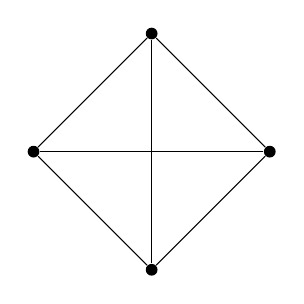
\begin{tikzpicture}[scale=1.5, every node/.style={circle, fill=black, inner sep=1.5pt}]
                \foreach \i in {1,...,4} {
                    \node (N\i) at ({360/4 * (\i - 1)}:1cm) {};
                }
                \foreach \i in {1,...,3} {
                    \pgfmathtruncatemacro{\next}{\i+1}
                    \foreach \j in {\next,...,4} {
                        \draw (N\i) -- (N\j);
                    }
                }
            \end{tikzpicture}
            \end{center}
            
            \item $K_5$
            
            The degree sequence for $K_5$ is \\(4, 4, 4, 4, 4). There is an Euler circuit and path.
            
            \begin{center}
            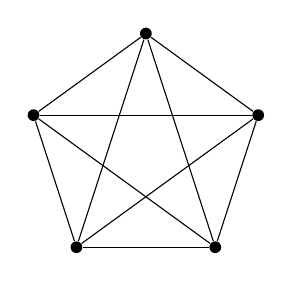
\begin{tikzpicture}[scale=1.5, every node/.style={circle, fill=black, inner sep=1.5pt}]
                \foreach \i in {1,...,5} {
                    \node (N\i) at ({360/5 * (\i - 1) - 270}:1cm) {};
                }
                \foreach \i in {1,...,4} {
                    \pgfmathtruncatemacro{\next}{\i+1}
                    \foreach \j in {\next,...,5} {
                        \draw (N\i) -- (N\j);
                    }
                }
            \end{tikzpicture}
            \end{center}
            
            \vspace{0.1pt}
            \item $K_{5,7}$
            
            The degree sequence for $K_{5,7}$ is \\(7, 7, 7, 7, 7, 5, 5, 5, 5, 5, 5, 5). There is neither an Euler circuit nor path.
            
            \begin{center}
            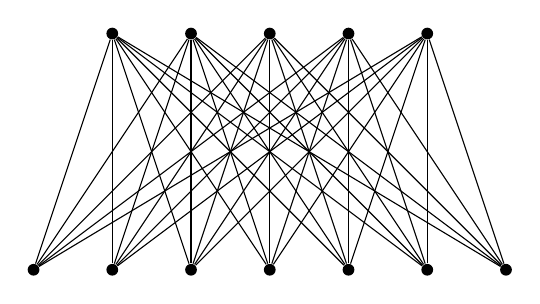
\begin{tikzpicture}[scale=1, every node/.style={circle, fill=black, inner sep=1.5pt}]
                \foreach \i in {1,...,5} {
                    \pgfmathsetmacro{\x}{-2 + (\i - 1)}
                    \node (A\i) at (\x, 2) {};
                }
                \foreach \j in {1,...,7} {
                    \pgfmathsetmacro{\x}{-3 + (\j - 1)}
                    \node (B\j) at (\x, -1) {};
                }
                \foreach \i in {1,...,5} {
                    \foreach \j in {1,...,7} {
                        \draw (A\i) -- (B\j);
                    }
                }
            \end{tikzpicture}
            \end{center}
        \end{enumerate}
        \end{minipage}
        \hfill
        \begin{minipage}[t]{0.48\textwidth}
        \begin{enumerate}[label=(\alph*), start=4]
            \item $K_{2,7}$
            
            The degree sequence for $K_{2,7}$ is \\(7, 7, 2, 2, 2, 2, 2, 2, 2). There is an Euler path, but no Euler circuit.
            
            \begin{center}
            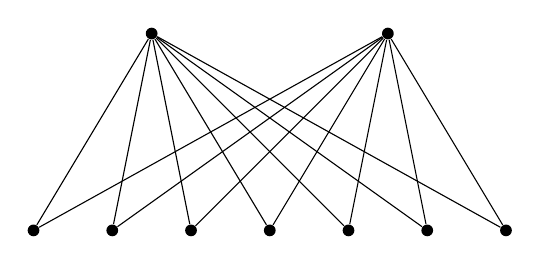
\begin{tikzpicture}[scale=1, every node/.style={circle, fill=black, inner sep=1.5pt}]
                \node (A1) at (-1.5, 1) {};
                \node (A2) at (1.5, 1) {};
                \foreach \i in {1,...,7} {
                    \pgfmathsetmacro{\x}{-3 + (\i - 1)}
                    \node (B\i) at (\x, -1.5) {};
                }
                \foreach \i in {1,2} {
                    \foreach \j in {1,...,7} {
                        \draw (A\i) -- (B\j);
                    }
                }
            \end{tikzpicture}
            \end{center}
            
            \vspace{10pt}
            \item $C_7$
            
            The degree sequence for $C_7$ is \\(2, 2, 2, 2, 2, 2, 2). There is an Euler circuit and path.
            
            \begin{center}
            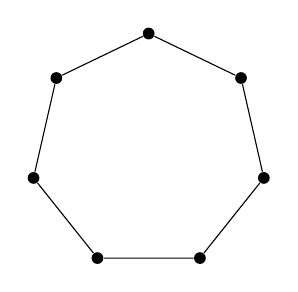
\begin{tikzpicture}[scale=1.5, every node/.style={circle, fill=black, inner sep=1.5pt}]
                \foreach \i in {1,...,7} {
                    \node (N\i) at ({360/7 * (\i - 1) + 90}:1cm) {};
                }
                \foreach \i in {1,...,6} {
                    \pgfmathtruncatemacro{\next}{\i+1}
                    \draw (N\i) -- (N\next);
                }
                \draw (N7) -- (N1);
            \end{tikzpicture}
            \end{center}
            
            \item $P_7$
            
            The degree sequence for $P_7$ is \\(2, 2, 2, 2, 2, 1, 1). There is an Euler path, but no Euler circuit.
            
            \begin{center}
            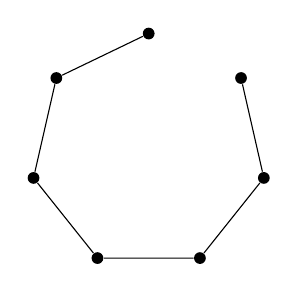
\begin{tikzpicture}[scale=1.5, every node/.style={circle, fill=black, inner sep=1.5pt}]
                \foreach \i in {1,...,7} {
                    \node (N\i) at ({360/7 * (\i - 1) + 90}:1cm) {};
                }
                \foreach \i in {1,...,6} {
                    \pgfmathtruncatemacro{\next}{\i+1}
                    \draw (N\i) -- (N\next);
                }
            \end{tikzpicture}
            \end{center}
        \end{enumerate}
        \end{minipage}
        \end{center}
        

    \item Consider the following graph:
    \begin{enumerate}[label=(\alph*)]
        \begin{multicols}{2}
        \item Find a Hamiltonian path. Can your path be extended to a Hamiltonian cycle?

        A Hamiltonian path is numbered from 1 to 11 in the figure.
        
        \item Is the graph bipartite? If so, how many vertices are in each ``part''?
        
        The graph is bipartite, each ``part'' is denoted by colors red and blue in the figure. One set contains 6 vertices, the other contains 5.
        \columnbreak

        \begin{figure}[H]
            \centering
            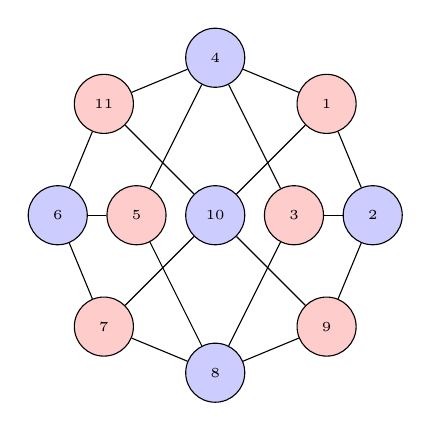
\begin{tikzpicture}[scale=2, every node/.style={draw, circle, minimum size=0.75cm}, font=\tiny]
    
                \node [fill=blue!20] (N1) at (0:1cm) {2};
                \node [fill=red!20] (N2) at (45:1cm) {1};
                \node [fill=blue!20] (N3) at (90:1cm) {4};
                \node [fill=red!20] (N4) at (135:1cm) {11};
                \node [fill=blue!20] (N5) at (180:1cm) {6};
                \node [fill=red!20] (N6) at (225:1cm) {7};
                \node [fill=blue!20] (N7) at (270:1cm) {8};
                \node [fill=red!20] (N8) at (315:1cm) {9};
                \node [fill=blue!20] (N9) at (0:0cm) {10};
                \node [fill=red!20] (N10) at (0:0.5cm) {3};
                \node [fill=red!20] (N11) at (0:-0.5cm) {5};
    
                \foreach \i in {1,...,7} {
                    \pgfmathtruncatemacro{\next}{\i+1}
                    \draw (N\i) -- (N\next);
                }
                % Finish cycle
                \draw (N8) -- (N1);
                % Horizontal
                \draw (N10) -- (N1);
                \draw (N11) -- (N5);
                % Cross
                \draw (N9) -- (N4);
                \draw (N9) -- (N2);
                \draw (N9) -- (N6);
                \draw (N9) -- (N8);
                % Diamond
                \draw (N10) -- (N3);
                \draw (N10) -- (N7);
                \draw (N11) -- (N3);
                \draw (N11) -- (N7);
         
            \end{tikzpicture}
        \end{figure}

    \end{multicols}
        
        \item Use your answer to part (b) to prove that the graph has no Hamilton cycle. 
        
        \begin{proof} By contradiction
           
            Assume the graph contains a Hamilton cycle.
            
            A Hamilton cycle visits every vertex exactly once, beginning and ending at the same vertex. 

            For a bipartite graph, this implies the Hamilton cycle must alternate between vertices in set $A$ and $B$, as no vertices in the same set are adjacent.

            For the given graph $|A| = |B|+ 1$.

            \underline{Case 1:} Start at a vertex in set A
       
            The cycle can then be described as:
            \[(a_1, b_1, a_2, b_2,..., a_{n - 1}, b_{n - 1}, a_n, a_1) \quad \text{ s.t. } a \in A \text{ and } b \in B\]

            But $a_1, a_n \in A$ and thus cannot be adjacent which is a contradiction.

            \underline{Case 2:} Start at a vertex in set B
            
            The cycle can then be described as:
            \[(b_1, a_1, b_2, a_2,..., b_{n - 1}, a_{n - 1}, a_n, b_1) \quad \text{ s.t. } a \in A \text{ and } b \in B\]
           
            Note vertex $b_n$ does not exist as $|A| = |B|+ 1$. $a_{n-1}, a_n \in A$ and thus cannot be adjacent which is a contradiction.

            Therefore by contradiction there cannot exist a Hamilton cycle.  
            
        \end{proof}

        
        \item Suppose you have a bipartite graph $G$ in which one part has at least two more vertices than the other. Prove that $G$ does not have a Hamilton path.

        \begin{proof}
            Let $G$ be a bipartite graph with sets $A$ and $B$ such that $|A| \ge |B| + 2$.
            
            Because G is bipartite, if a Hamilton path exists, the vertices in the path will alternate between vertices in A and vertices in B.

            In the minimum case: 
            \[A = \{a_1, a_2, ... , a_n\} \text{ and } B = \{b_1, b_2, ..., b_{n - 2}\} \quad \text{ if } |A| = |B| + 2\]

            We pair up vertices from sets A and B to create a path.
        
            \underline{Case 1:} Start at a vertex in set A

            The path can be described as:
            \[(a_1, b_1, a_2, b_2, \ldots , a_{n - 2}, b_{n - 2}, a_{n - 1}, a_{n}) \quad \text{ s.t. } a \in A \text{ and } b \in B\]
           
            But $a_{n - 1}, a_{n} \in A$ and thus cannot be adjacent which is a contradiction.
            
            \underline{Case 2:} Start at a vertex in set B
            
            The path can be described as:
            \[(b_1, a_1, b_2, a_2, ... , b_{n - 2}, a_{n - 2}, a_{n - 1}, a_{n}) \quad \text{ s.t. } a \in A \text{ and } b \in B\]
            
            But $a_{n - 2}, a_{n - 1}, a_{n} \in A$ and thus cannot be adjacent which is a contradiction.

            In any case where $|A| > |B| + 2$ A would have more vertices and more would be unpaired.

            Therefore by contradiction there cannot exist a Hamilton path.
        \end{proof}
    \end{enumerate}

    

    \item Find a matching of the bipartite graphs below or explain why no matching exists.
    \begin{multicols}{3}
    
    \begin{center}
        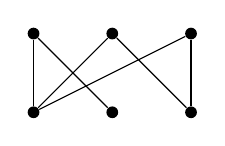
\begin{tikzpicture}[scale=1, every node/.style={circle, fill=black, inner sep=1.5pt}]
            \foreach \i in {1,...,3} {
                \pgfmathsetmacro{\x}{(\i - 1)}
                \node  (A\i) at (\x, 1) {};
            }
            \foreach \j in {1,...,3} {
                \pgfmathsetmacro{\x}{(\j - 1)}
                \node (B\j) at (\x, 0) {};
            }
            \draw (A1) -- (B1);
            \draw (A2) -- (B1);
            \draw (A3) -- (B1);
            \draw (A1) -- (B2);
            \draw (A2) -- (B3);
            \draw (A3) -- (B3);

        \end{tikzpicture}
    \end{center}

    \begin{center}
        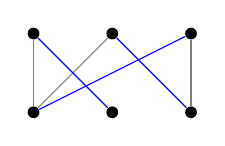
\begin{tikzpicture}[scale=1, every node/.style={circle, fill=black, inner sep=1.5pt}]
            \foreach \i in {1,...,3} {
                \pgfmathsetmacro{\x}{(\i - 1)}
                \node  (A\i) at (\x, 1) {};
            }
            \foreach \j in {1,...,3} {
                \pgfmathsetmacro{\x}{(\j - 1)}
                \node (B\j) at (\x, 0) {};
            }
            \draw [draw=gray] (A1) -- (B1);
            \draw [draw=gray] (A2) -- (B1);
            \draw [draw=blue] (A3) -- (B1);
            \draw [draw=blue] (A1) -- (B2);
            \draw [draw=blue] (A2) -- (B3);
            \draw [draw=gray] (A3) -- (B3);

        \end{tikzpicture}
    \end{center}

    \columnbreak

    \begin{center}
        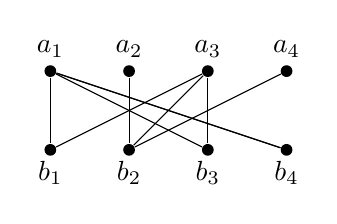
\begin{tikzpicture}[scale=1, every node/.style={circle, fill=black, inner sep=1.5pt}]
            \foreach \i in {1,...,4} {
                \pgfmathsetmacro{\x}{(\i - 1)}
                \node  (A\i) at (\x, 1) {};
                \node[draw=none, fill=none, anchor=south] at (\x, 1) {$a_{\i}$};
            }
            \foreach \j in {1,...,4} {
                \pgfmathsetmacro{\x}{(\j - 1)}
                \node (B\j) at (\x, 0) {};
                \node[draw=none, fill=none, anchor=north] at (\x, 0) {$b_{\j}$};
            }

            \draw (A1) -- (B1);
            \draw (A2) -- (B2);
            \draw (A3) -- (B3);
            \draw (A1) -- (B3);
            \draw (A3) -- (B1);
            \draw (A4) -- (B2);
            \draw (A1) -- (B4);
            \draw (A1) -- (B4);
            \draw (A3) -- (B2);
`'
        \end{tikzpicture}
    \end{center}
    No matching exists because $a_2$ and $a_4$ are only adjacent to $b_2$.

    \columnbreak
    
    
    \begin{center}
        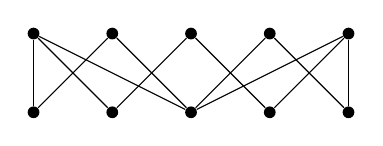
\begin{tikzpicture}[scale=1, every node/.style={circle, fill=black, inner sep=1.5pt}]
            \foreach \i in {1,...,5} {
                \pgfmathsetmacro{\x}{(\i - 1)}
                \node  (A\i) at (\x, 1) {};
            }
            \foreach \j in {1,...,5} {
                \pgfmathsetmacro{\x}{(\j - 1)}
                \node (B\j) at (\x, 0) {};
            }

            \draw  (A1) -- (B1);
            \draw  (A5) -- (B5);
            \draw  (A1) -- (B3);
            \draw  (A5) -- (B3);
            \foreach \i in {1,...,4} {
                    \pgfmathtruncatemacro{\next}{\i+1}
                    \draw (A\i) -- (B\next);
            }

            \foreach \i in {1,...,4} {
                    \pgfmathtruncatemacro{\next}{\i+1}
                    \draw (B\i) -- (A\next);
            }

        \end{tikzpicture}
    \end{center}

    \begin{center}
        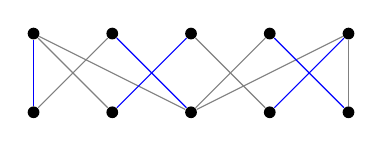
\begin{tikzpicture}[scale=1, every node/.style={circle, fill=black, inner sep=1.5pt}]
            \foreach \i in {1,...,5} {
                \pgfmathsetmacro{\x}{(\i - 1)}
                \node  (A\i) at (\x, 1) {};
            }
            \foreach \j in {1,...,5} {
                \pgfmathsetmacro{\x}{(\j - 1)}
                \node (B\j) at (\x, 0) {};
            }

            \draw [draw=blue] (A1) -- (B1);
            \draw [draw=gray] (A5) -- (B5);
            \draw [draw=gray] (A1) -- (B3);
            \draw [draw=gray] (A5) -- (B3);
            \draw [draw=gray] (A1) -- (B2);
            \draw [draw=blue] (A2) -- (B3);
            \draw [draw=gray] (A3) -- (B4);
            \draw [draw=blue] (A4) -- (B5);
            \draw [draw=gray] (B1) -- (A2);
            \draw [draw=blue] (B2) -- (A3);
            \draw [draw=gray] (B3) -- (A4);
            \draw [draw=blue] (B4) -- (A5);

        \end{tikzpicture}
    \end{center}
\end{multicols}
    
    
    \item What is the smallest number of colors you need to properly color the vertices of $K_{5,7}$?
        
          Two as it is a bipartite graph.

          \begin{center}
            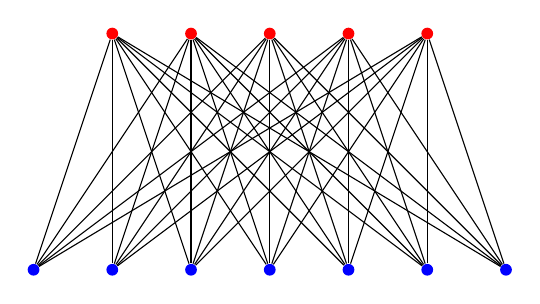
\begin{tikzpicture}[scale=1, every node/.style={circle, inner sep=1.5pt}]
                \foreach \i in {1,...,5} {
                    \pgfmathsetmacro{\x}{-2 + (\i - 1)}
                    \node  [fill=red] (A\i) at (\x, 2) {};
                }
                \foreach \j in {1,...,7} {
                    \pgfmathsetmacro{\x}{-3 + (\j - 1)}
                    \node (B\j) [fill=blue] at (\x, -1) {};
                }
                \foreach \i in {1,...,5} {
                    \foreach \j in {1,...,7} {
                        \draw (A\i) -- (B\j);
                    }
                }
            \end{tikzpicture}
            \end{center}
    \item Draw a graph with chromatic number 5. Could your graph be planar? Explain.
    No because by the Four Color Theorem which states that ``If $G$ is a planar graph, then the chromatic number of $G$ is less than or equal to 4.'' 

    \begin{center}
        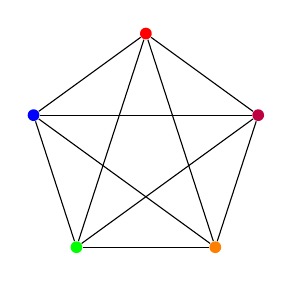
\begin{tikzpicture}[scale=1.5, every node/.style={circle, fill=black, inner sep=1.5pt}]
            \node [fill=red]    (N1) at (-270:1cm) {};
            \node [fill=blue]   (N2) at (-198:1cm) {};
            \node [fill=green]  (N3) at (-126:1cm) {};
            \node [fill=orange] (N4) at (-54:1cm)  {};
            \node [fill=purple] (N5) at (18:1cm)   {};
            \foreach \i in {1,...,4} {
                        \pgfmathtruncatemacro{\next}{\i+1}
                        \foreach \j in {\next,...,5} {
                            \draw (N\i) -- (N\j);
                        }
                    }
        \end{tikzpicture}
    \end{center}


    \item The local Entomology Club has six work groups, each meeting once a month. How many different meeting times must be used to ensure that no member is scheduled to attend two meetings at the same time if the work groups consist of the following members?
    
    W1 = \{John, Voormann, Ringo\}\\
    W2 = \{Voormann, George, Paul\}\\
    W3 = \{John, Paul, Ringo\}\\
    W4 = \{George, Paul, Ringo\}\\
    W5 = \{John, Voormann\}\\
    W6 = \{Voormann, Paul, Ringo\}\\
\end{enumerate}


% \begin{tikzpicture}[scale=2, every node/.style={draw, circle, minimum size=0.75cm}, font=\tiny]
%     \node (W1) at (0:1cm) {W1};
%     \node (W2) at (60:1cm) {W2};
%     \node (W3) at (120:1cm) {W3};
%     \node (W4) at (180:1cm) {W4};
%     \node (W5) at (240:1cm) {W5};
%     \node (W6) at (300:1cm) {W6};

%     % John
%     \draw (W3) -- (W1);
%     \draw (W1) -- (W5);
%     \draw (W5) -- (W3);

%     % Voormann
%     \draw (W2) -- (W1);
%     \draw (W1) -- (W6);
%     \draw (W5) -- (W6);
%     \draw (W5) -- (W2);
%     \draw (W1) -- (W5);
%     \draw (W6) -- (W2);

%     % Ringo
%     \draw (W3) -- (W1);
%     \draw (W3) -- (W6);
%     \draw (W3) -- (W4);
%     \draw (W4) -- (W1);
%     \draw (W4) -- (W6);
%     \draw (W1) -- (W6);

%     % George
%     \draw (W4) -- (W2);

%     % Paul
%     \draw (W3) -- (W2);
%     \draw (W3) -- (W4);
%     \draw (W3) -- (W6);
%     \draw (W2) -- (W6);
%     \draw (W2) -- (W4);
%     \draw (W4) -- (W6);

% \end{tikzpicture}



\begin{center}
    % Row 1
    \begin{minipage}{0.45\textwidth}
    \centering
    {John}\\[5pt]
    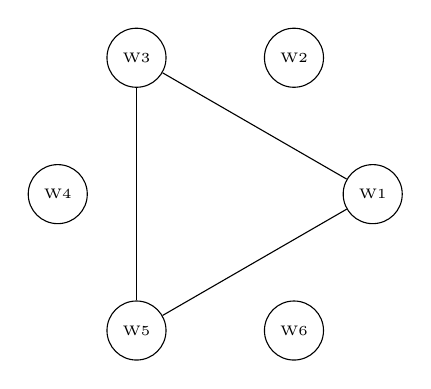
\begin{tikzpicture}[scale=2, every node/.style={draw, circle, minimum size=0.75cm}, font=\tiny]
        \node (W1) at (0:1cm) {W1};
        \node (W2) at (60:1cm) {W2};
        \node (W3) at (120:1cm) {W3};
        \node (W4) at (180:1cm) {W4};
        \node (W5) at (240:1cm) {W5};
        \node (W6) at (300:1cm) {W6};
    
        \draw (W3) -- (W1);
        \draw (W1) -- (W5);
        \draw (W5) -- (W3);
    \end{tikzpicture}
    \end{minipage}
    \hfill
    \begin{minipage}{0.45\textwidth}
    \centering
    {Voormann}\\[5pt]
    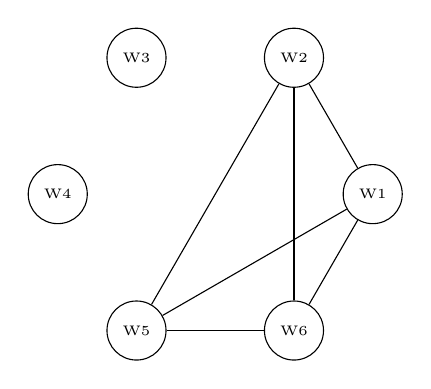
\begin{tikzpicture}[scale=2, every node/.style={draw, circle, minimum size=0.75cm}, font=\tiny]
        \node (W1) at (0:1cm) {W1};
        \node (W2) at (60:1cm) {W2};
        \node (W3) at (120:1cm) {W3};
        \node (W4) at (180:1cm) {W4};
        \node (W5) at (240:1cm) {W5};
        \node (W6) at (300:1cm) {W6};
    
        \draw (W2) -- (W1);
        \draw (W1) -- (W6);
        \draw (W5) -- (W6);
        \draw (W5) -- (W2);
        \draw (W1) -- (W5);
        \draw (W6) -- (W2);
    \end{tikzpicture}
    \end{minipage}
    
    \vspace{1cm}
    
    % Row 2
    \begin{minipage}{0.45\textwidth}
    \centering
    {Ringo}\\[5pt]
    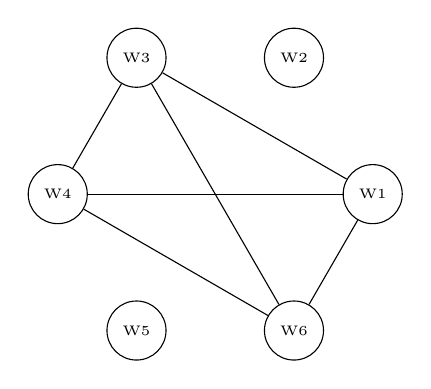
\begin{tikzpicture}[scale=2, every node/.style={draw, circle, minimum size=0.75cm}, font=\tiny]
        \node (W1) at (0:1cm) {W1};
        \node (W2) at (60:1cm) {W2};
        \node (W3) at (120:1cm) {W3};
        \node (W4) at (180:1cm) {W4};
        \node (W5) at (240:1cm) {W5};
        \node (W6) at (300:1cm) {W6};
    
        \draw (W3) -- (W1);
        \draw (W3) -- (W6);
        \draw (W3) -- (W4);
        \draw (W4) -- (W1);
        \draw (W4) -- (W6);
        \draw (W1) -- (W6);
    \end{tikzpicture}
    \end{minipage}
    \hfill
    \begin{minipage}{0.45\textwidth}
    \centering
    {George}\\[5pt]
    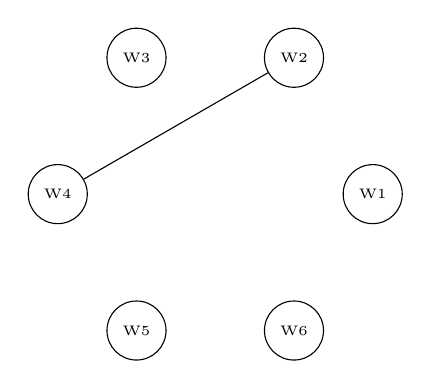
\begin{tikzpicture}[scale=2, every node/.style={draw, circle, minimum size=0.75cm}, font=\tiny]
        \node (W1) at (0:1cm) {W1};
        \node (W2) at (60:1cm) {W2};
        \node (W3) at (120:1cm) {W3};
        \node (W4) at (180:1cm) {W4};
        \node (W5) at (240:1cm) {W5};
        \node (W6) at (300:1cm) {W6};
    
        \draw (W4) -- (W2);
    \end{tikzpicture}
    \end{minipage}
    
    \vspace{1cm}
    
    % Row 3
    \begin{minipage}{0.45\textwidth}
    \centering
    {Paul}\\[5pt]
    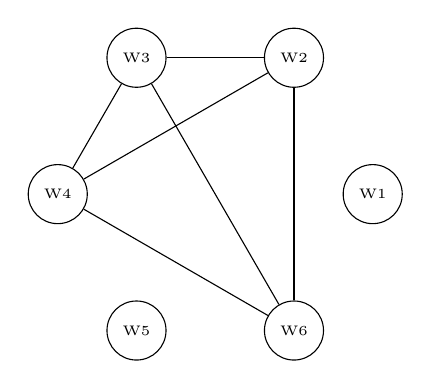
\begin{tikzpicture}[scale=2, every node/.style={draw, circle, minimum size=0.75cm}, font=\tiny]
        \node (W1) at (0:1cm) {W1};
        \node (W2) at (60:1cm) {W2};
        \node (W3) at (120:1cm) {W3};
        \node (W4) at (180:1cm) {W4};
        \node (W5) at (240:1cm) {W5};
        \node (W6) at (300:1cm) {W6};
    
        \draw (W3) -- (W2);
        \draw (W3) -- (W4);
        \draw (W3) -- (W6);
        \draw (W2) -- (W6);
        \draw (W2) -- (W4);
        \draw (W4) -- (W6);
    \end{tikzpicture}
    \end{minipage}
 \end{center}

 \vspace*{-0.4 cm}
 Eight meeting times are required.
    

\end{document}